\documentclass[tikz,border=8pt]{standalone}
% Shared look for every TikZ diagram. Load with % Shared look for every TikZ diagram. Load with % Shared look for every TikZ diagram. Load with \input{../../tools/tikz-style.tex}
\usepackage[T1]{fontenc}
\usepackage{lmodern}
\renewcommand{\sfdefault}{lmr}  % diagrams use the same serif as the text
\usetikzlibrary{arrows.meta, positioning, shapes.geometric, calc, fit, backgrounds}
\definecolor{cblue}{HTML}{4C78A8}
\definecolor{corange}{HTML}{F58518}
\definecolor{cgreen}{HTML}{54A24B}
\definecolor{cred}{HTML}{E45756}
\definecolor{cpurple}{HTML}{B279A2}
\definecolor{cgrey}{HTML}{6B6B6B}
\tikzset{
  every picture/.style={font=\sffamily, line width=1.2pt},
  box/.style={draw=#1, fill=#1!12, rounded corners=4pt, align=center, inner sep=7pt, minimum height=1.1cm},
  box/.default=cgrey,
  arrow/.style={-{Stealth[length=3mm]}, draw=cgrey, line width=1.4pt},
  title/.style={font=\sffamily\bfseries\Large},
  note/.style={font=\sffamily\small, text=cgrey, align=center},
}
\AtBeginDocument{\hyphenpenalty=10000 \exhyphenpenalty=10000}

\usepackage[T1]{fontenc}
\usepackage{lmodern}
\renewcommand{\sfdefault}{lmr}  % diagrams use the same serif as the text
\usetikzlibrary{arrows.meta, positioning, shapes.geometric, calc, fit, backgrounds}
\definecolor{cblue}{HTML}{4C78A8}
\definecolor{corange}{HTML}{F58518}
\definecolor{cgreen}{HTML}{54A24B}
\definecolor{cred}{HTML}{E45756}
\definecolor{cpurple}{HTML}{B279A2}
\definecolor{cgrey}{HTML}{6B6B6B}
\tikzset{
  every picture/.style={font=\sffamily, line width=1.2pt},
  box/.style={draw=#1, fill=#1!12, rounded corners=4pt, align=center, inner sep=7pt, minimum height=1.1cm},
  box/.default=cgrey,
  arrow/.style={-{Stealth[length=3mm]}, draw=cgrey, line width=1.4pt},
  title/.style={font=\sffamily\bfseries\Large},
  note/.style={font=\sffamily\small, text=cgrey, align=center},
}
\AtBeginDocument{\hyphenpenalty=10000 \exhyphenpenalty=10000}

\usepackage[T1]{fontenc}
\usepackage{lmodern}
\renewcommand{\sfdefault}{lmr}  % diagrams use the same serif as the text
\usetikzlibrary{arrows.meta, positioning, shapes.geometric, calc, fit, backgrounds}
\definecolor{cblue}{HTML}{4C78A8}
\definecolor{corange}{HTML}{F58518}
\definecolor{cgreen}{HTML}{54A24B}
\definecolor{cred}{HTML}{E45756}
\definecolor{cpurple}{HTML}{B279A2}
\definecolor{cgrey}{HTML}{6B6B6B}
\tikzset{
  every picture/.style={font=\sffamily, line width=1.2pt},
  box/.style={draw=#1, fill=#1!12, rounded corners=4pt, align=center, inner sep=7pt, minimum height=1.1cm},
  box/.default=cgrey,
  arrow/.style={-{Stealth[length=3mm]}, draw=cgrey, line width=1.4pt},
  title/.style={font=\sffamily\bfseries\Large},
  note/.style={font=\sffamily\small, text=cgrey, align=center},
}
\AtBeginDocument{\hyphenpenalty=10000 \exhyphenpenalty=10000}

\begin{document}
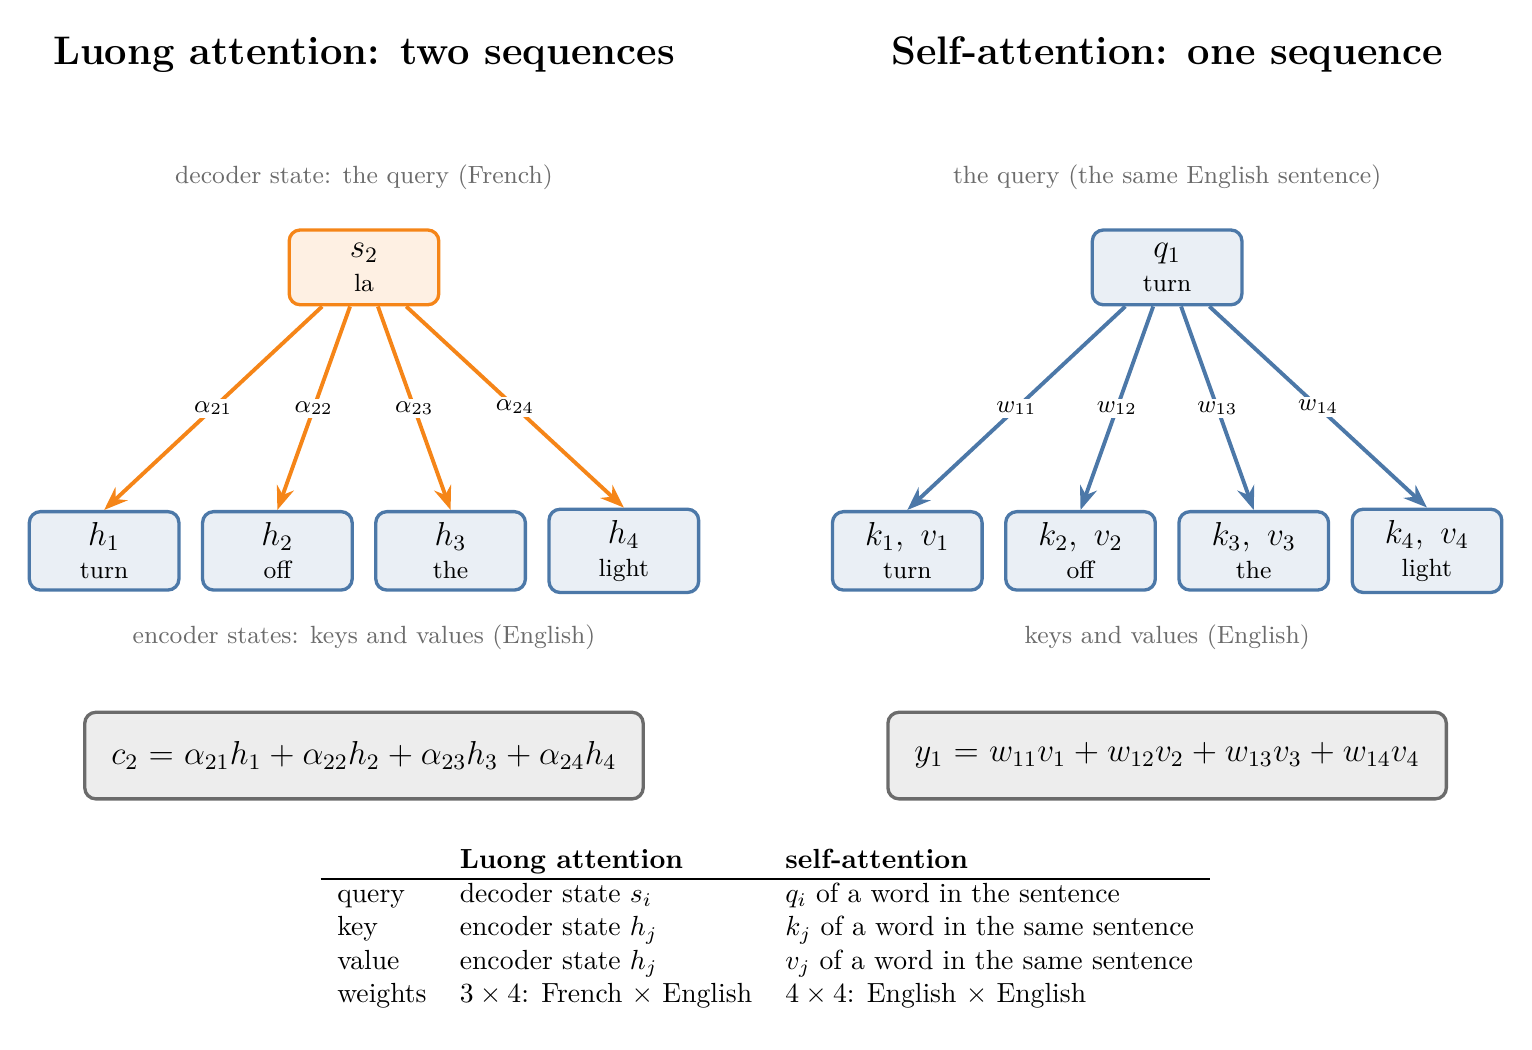
\begin{tikzpicture}[every node/.append style={font=\sffamily\large},
  w/.style={box=#1, minimum width=1.9cm, inner sep=4pt, minimum height=0.95cm}]
  % ---------- left: Luong attention between two sequences
  \node[title] at (3.3, 6.3) {Luong attention: two sequences};
  \foreach \t/\x [count=\j] in {turn/0, off/2.2, the/4.4, light/6.6}
    \node[w=cblue] (h\j) at (\x, 0) {$h_{\j}$\\[-2pt]\small \t};
  \node[note] at (3.3, -1.1) {encoder states: keys and values (English)};
  \node[w=corange] (s) at (3.3, 3.6) {$s_2$\\[-2pt]\small la};
  \node[note] at (3.3, 4.75) {decoder state: the query (French)};
  \foreach \j/\a in {1/0.23, 2/0.26, 3/0.26, 4/0.25}
    \draw[arrow, draw=corange] (s) -- node[fill=white, inner sep=1pt, font=\sffamily\small] {$\alpha_{2\j}$} (h\j.north);
  \node[box=cgrey, text width=6.6cm] at (3.3, -2.6) {$c_2 = \alpha_{21}h_1 + \alpha_{22}h_2 + \alpha_{23}h_3 + \alpha_{24}h_4$};
  % ---------- right: self-attention within one sequence
  \begin{scope}[xshift=10.2cm]
  \node[title] at (3.3, 6.3) {Self-attention: one sequence};
  \foreach \t/\x [count=\j] in {turn/0, off/2.2, the/4.4, light/6.6}
    \node[w=cblue] (k\j) at (\x, 0) {$k_{\j},\ v_{\j}$\\[-2pt]\small \t};
  \node[note] at (3.3, -1.1) {keys and values (English)};
  \node[w=cblue] (q) at (3.3, 3.6) {$q_1$\\[-2pt]\small turn};
  \node[note] at (3.3, 4.75) {the query (the same English sentence)};
  \foreach \j in {1,2,3,4}
    \draw[arrow, draw=cblue] (q) -- node[fill=white, inner sep=1pt, font=\sffamily\small] {$w_{1\j}$} (k\j.north);
  \node[box=cgrey, text width=6.6cm] at (3.3, -2.6) {$y_1 = w_{11}v_1 + w_{12}v_2 + w_{13}v_3 + w_{14}v_4$};
  \end{scope}
  % ---------- roles
  \node[align=left, font=\sffamily, anchor=north] at (8.4, -3.6) {
  \begin{tabular}{lll}
   & \textbf{Luong attention} & \textbf{self-attention}\\ \hline
   query & decoder state $s_i$ & $q_i$ of a word in the sentence\\
   key & encoder state $h_j$ & $k_j$ of a word in the same sentence\\
   value & encoder state $h_j$ & $v_j$ of a word in the same sentence\\
   weights & $3 \times 4$: French $\times$ English & $4 \times 4$: English $\times$ English\\
  \end{tabular}};
\end{tikzpicture}
\end{document}
